%%%% SIGNAL SECTION %%%%
\section{MCS Performance on Muons from numuCC Events in MicroBooNE Data}\label{data_performance_section}

\subsection{Input sample}
reference CCInclusive technote, good runs list, no EXT data used only BNB. cosmic backgrounds are low after event selection (quantify this probably). especially low after hand scanning too

\subsection{Event selection}
\begin{enumerate}
\item describe the event selection, 2 tracks at vertex, etc etc.
\item state we take tracks fully contained in fiducial volume, longer than 1 meter
\item state that broken tracks are still present so we do hand scanning
\item describe hand scanning, include pictures of event displays like Figure \ref{bad_evd_fig_1}.
\end{enumerate}

\begin{figure}[h!]
\begin{center}
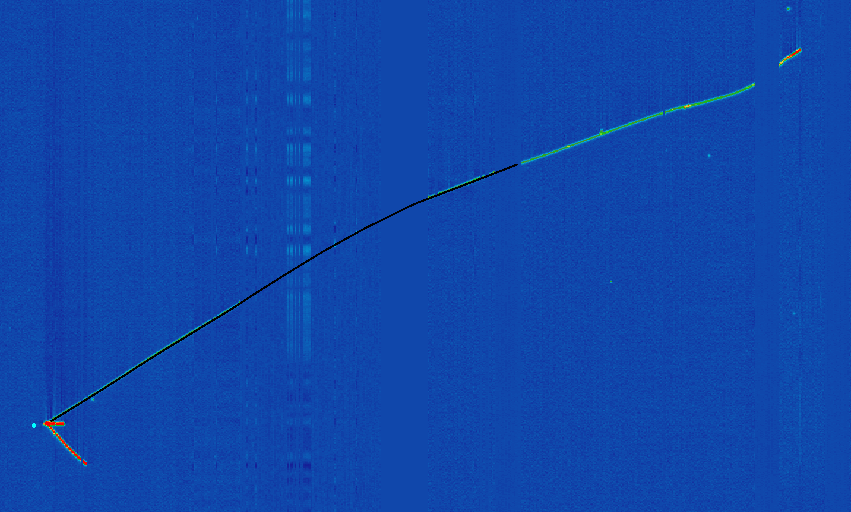
\includegraphics[width=100mm]{Figures/bad_evd_1.png}
\end{center}
\caption{\textit{bad evd caption}}
\label{bad_evd_fig_1}
\end{figure}

\subsection{Performance}
\begin{enumerate}
\item plot of scattering angle / RMS (RMS from MCS energy, or range energy). hopefully this agrees with the corresponding plot in the MC section. maybe put them on the same plot?
\item plot of MCS energy vs range
\item energy resolution in terms of range energy. hopefully this agrees with the corresponding plot in the MC section. maybe put them on the same plot?
\end{enumerate}